Examine the marginal normality of the observations on variables $X_{1}, X_{2}, \dots, X_{5}$ for the
multiple-sclerosis data in Table 1.6. Treat the non-multiple-sclerosis and multiple-sclerosis
groups separately. Use whatever methodology, including transformations, you feel is appropriate.
\newline There are 10 vectors that need to be checked and I'll pick an $\alpha\text{-level}$ of 0.01 for our tests.
\begin{center}
    \begin{tabular}{lcc}
        \hline % chktex 44
        $x_{i}$ & MS Negative $r_{Q}$ & MS Positive $r_{Q}$ \\
        \hline % chktex 44
        Age                      & 0.9448 & 0.9714 \\
        $S1L + S1R$              & 0.9613 & 0.9703 \\
        $\left|S1L - S1R\right|$ & 0.9558 & 0.7952 \\
        $S2L + S2R$              & 0.9757 & 0.9787 \\
        $\left|S2L - S2R\right|$ & 0.9445 & 0.8413 \\
        \hline % chktex 44
    \end{tabular}
\end{center}
The correlation coefficients for the Q-Q plots for all the variables are in the table above. The MS positive group has low $r_{Q}$ values for variables $\left|S1L - S1R\right|$ and $\left|S2L - S2R\right|$. For MS negative, variable $\left|S2L - S2R\right|$ has the lowest $r_{Q}$ value within group.

From Table 4.2 for the negative MS group the sample size of 69 and significance level $\alpha = 0.01$, the critical point would be somewhere within 0.9720 and 9771. Instead of relying on the table, performing 1M simulations, the value found is 0.9752. Based on this value, only the variable $S2L + S2R$ for the negative MS group would be considered normally distributed. Variables $x_{1}$, $x_{2}$, $x_{3}$, and $x_{5}$ are in need of a transformation. The Q-Q plots for each of the five variables is below.

\begin{center}
    \begin{figure}[H]
        \centering
        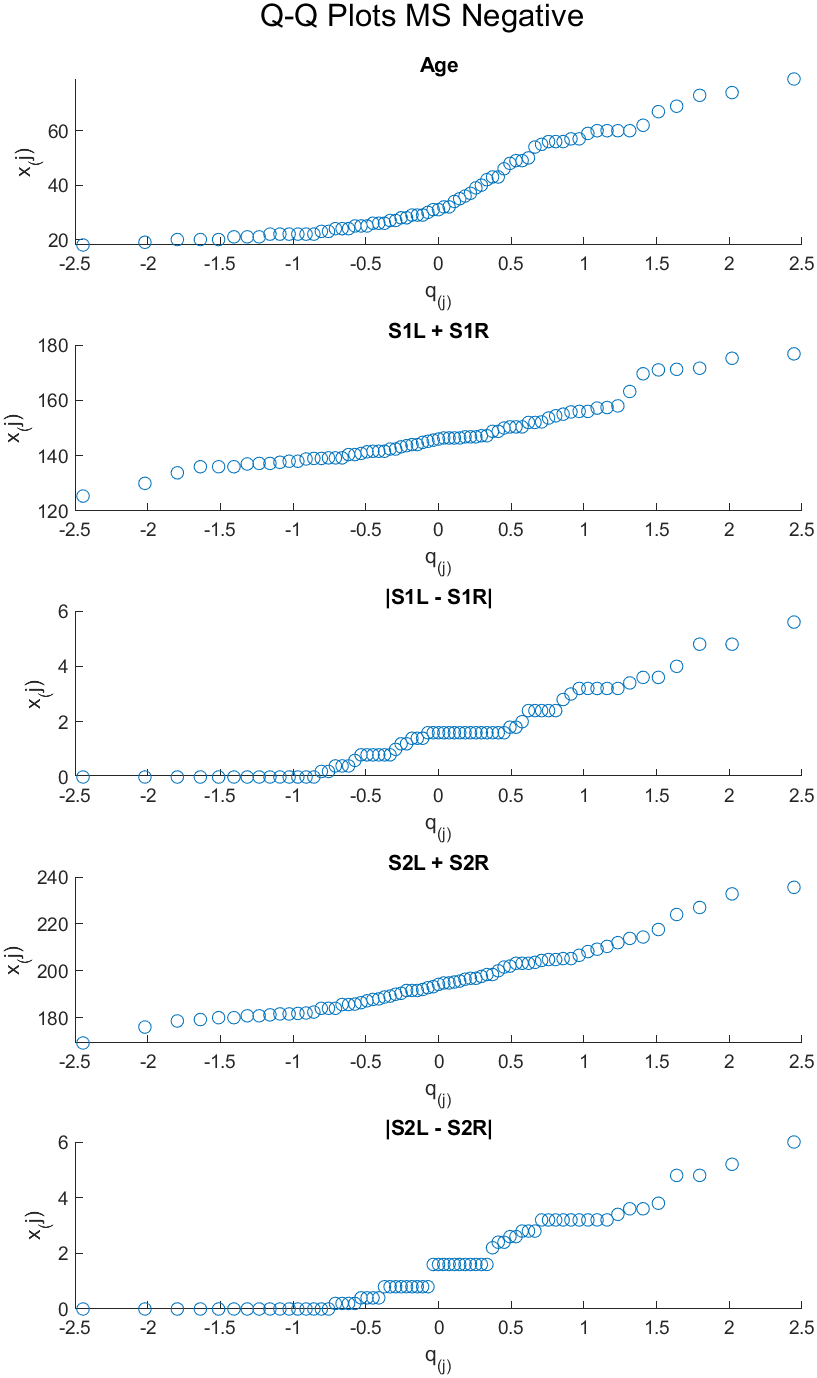
\includegraphics[scale=0.6]{./matlab/chapter-4/sol4.31.qq.msneg.png}
    \end{figure}
\end{center}

For the positive MS group the sample size is 29, so from Table 4.2 where the significance level is 0.01, the critical point is slightly less than 0.9479, but larger than 0.9410. Performing the simulation for sample size 29 and 1M replications, the critical point found was 0.9475. In this case, only $x_{3}$ and $x_{5}$, that is, $\left|S1L - S1R\right|$ and $\left|S2L - S2R\right|$, would be considered not to be normally distributed and need a transformation. The Q-Q plots for the variables in the MS positive group are below.

\begin{center}
    \begin{figure}[H]
        \centering
        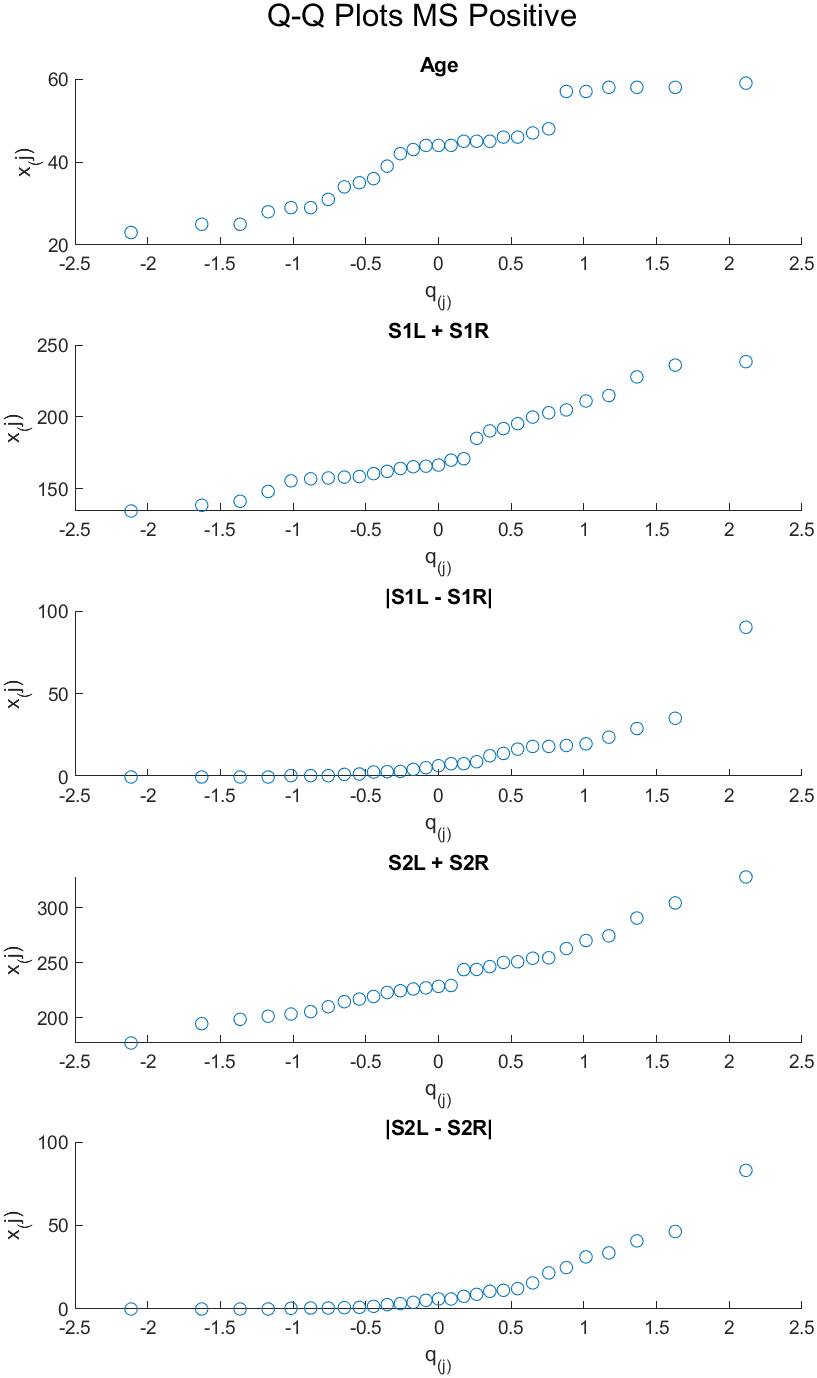
\includegraphics[scale=0.6]{./matlab/chapter-4/sol4.31.qq.mspos.png}
    \end{figure}
\end{center}

\begin{table}[H]
    \caption*{Univariate Power Transformation}
    \centering
    \begin{tabular}{lcc}
        \hline % chktex 44
                & MS Negative                        & MS Positive \\
        $x_{i}$ & $\max\{\ell\left(\lambda\right)\}$ & $\max\{\ell\left(\lambda\right)\}$ \\
        \hline % chktex 44
        Age                      & -0.4910     & \textemdash\\
        $S1L + S1R$              & -3.5371     & \textemdash\\
        $\left|S1L - S1R\right|$ & 0.2305      & 0.2104     \\
        $S2L + S2R$              & \textemdash~& \textemdash\\
        $\left|S2L - S2R\right|$ & 0.1904      & 0.1904     \\
        \hline % chktex 44        
    \end{tabular}
\end{table}

The results of performing the univariate power transformation are in the table above. I left the power transformation plots out, but copies can be found in the \texttt{matlab} folder. For the MS Negative group, rounding things off, it looks like Age could use a negative square-root transformation. The variable $S1L + S1R$ could use a transformation of -3.5. Variable, $\left|S1L - S1R\right|$, rounds to  $1/4$ and $1/5$ for $\left|S2L - S2R\right|$. For the MS positive data, again, $\left|S1L - S1R\right|$ is transformed using a power of $1/4$ and $\left|S2L - S2R\right|$ a power of $1/5$.

\begin{table}[H]
    \caption*{Q-Q Correlation Transformed Data}
    \centering
    \begin{tabular}{lcc}
        \hline % chktex 44
        & MS Negative                        & MS Positive \\
        $x_{i}$ & Transformed $r_{Q}$ & Transformed $r_{Q}$ \\
        \hline % chktex 44
        Age                      & 0.9694      & \textemdash\\
        $S1L + S1R$              & 0.9878      & \textemdash\\
        $\left|S1L - S1R\right|$ & 0.8888      & 0.9679     \\
        $S2L + S2R$              & \textemdash~& \textemdash\\
        $\left|S2L - S2R\right|$ & 0.8852      & 0.9651     \\
        \hline % chktex 44
    \end{tabular}
\end{table}

Computing the Q-Q values on the transformed data seems to have normalized the MS positive group columns $\left|S1L - S1R\right|$ and $\left|S2L - S2R\right|$. 
Both values are greater than the critical point value of 0.9475. For the MS negative group, the variable $S1L + S1R$ looks okay now, and has a Q-Q correlation value (0.9878) larger than the 0.01-level critical value of 0.9752. 
For the MS negative group, transforming variable Age was helpful, but the Q-Q correlation value (0.9694) is still not quite larger than the critical value. 
Lastly, for the MS negative group, transforming variables $\left|S1L - S1R\right|$ and $\left|S2L - S2R\right|$, the results are worse than the raw data. 
This might be due to the number of 0 values. For these two variables the MS negative group has 20\% to 25\% zero values, but the MS positive group it's around 13\%, so people without MS have less of an absolute difference between left and right eye than people with MS. 
Maybe instead we could use an factor variable to indicate if the absolute difference is 0 or not.
